El algoritmo es muy simple: al principio anotamos todos los números entre 2 y $n$. Marcamos todos los 
múltiplos propios de 2 (ya que 2 es el número primo más pequeño) como compuestos. Un múltiplo propio 
de un número $x$, es un número mayor que $x$ y divisible por $x$. Luego encontramos el siguiente 
número que no ha sido marcado como compuesto, en este caso es 3. Lo que significa que 3 es primo y 
marcamos todos los múltiplos propios de 3 como compuestos. El siguiente número sin marcar es 5, que 
es el siguiente número primo, y marcamos todos los múltiplos propios del mismo. Y continuamos este 
procedimiento hasta que hayamos procesado todos los números de la fila.

En la siguiente imagen puedes ver una visualización del algoritmo para calcular todos los números primos en el rango $[1; 16]$. Se puede ver que muy a menudo marcamos los números como compuestos varias veces.

% TODO: \usepackage{graphicx} required
\begin{figure}[h!]
	\centering
	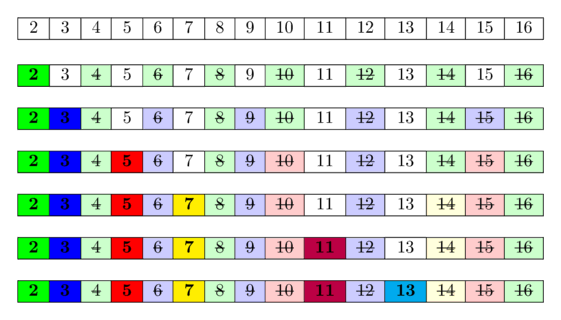
\includegraphics[width=1\linewidth]{img/sieve_eratosthenes}

	\label{fig:sieveeratosthenes}
\end{figure}


La idea detrás es la siguiente: un número es primo si ninguno de los números primos más pequeños lo divide. Dado que iteramos sobre los números primos en orden, ya marcamos todos los números que son divisibles por al menos uno de los números primos como divisibles. Por lo tanto, si llegamos a una celda y no está marcada, entonces no es divisible por ningún número primo menor y, por lo tanto, tiene que ser primo.


\subsection{Diferentes optimizaciones de la criba de  Eratóstenes}

La mayor debilidad del algoritmo es que camina a lo largo de la memoria varias veces, manipulando únicamente elementos individuales. Esto no es muy amigable con el caché. Y por eso, la constante que se esconde en $O(n \log \log n)$ es comparativamente grande.

Además, la memoria consumida es un cuello de botella para las grandes $n$.

Los métodos presentados a continuación nos permiten reducir la cantidad de operaciones realizadas, así como acortar notablemente la memoria consumida.

\subsubsection{Iterar hasta la raíz}

Obviamente, para encontrar todos los números primos hasta $n$, bastará con realizar el cribado únicamente por los números primos, que no superen la raíz de $n$.

\subsubsection{Iterar solo por los números impares}

Dado que todos los números pares (excepto $2$) son compuestos, podemos dejar de verificar los números pares. En cambio, necesitamos operar sólo con números impares.

\subsubsection{Reducir la memoria consumida}

Debemos notar que estas dos optimizaciones de la criba de Eratóstenes usan $n$ bits de memoria mediante el uso de la estructura de datos \textbf{vector<bool>}.  \textbf{vector<bool>} no es un contenedor normal que almacena una serie de \textbf{bool} (como en la mayoría de las arquitecturas de computadora, \textbf{bool} ocupa un byte de memoria). Es una especialización de optimización de memoria de \textbf{vector<T>}, que solo consume $\frac{N}{8}$ bytes de memoria.

Las arquitecturas de procesadores modernas funcionan mucho más eficientemente con bytes que con bits, ya que normalmente no pueden acceder a los bits directamente. Entonces, debajo \textbf{vector<bool>} almacena los bits en una gran memoria continua, accede a la memoria en bloques de unos pocos bytes y extrae/establece los bits con operaciones de bits como enmascaramiento de bits y desplazamiento de bits.

Debido a eso, hay una cierta sobrecarga cuando lees o escribes bits con a \textbf{vector<bool>} y, muy a menudo, usar a \textbf{vector<char>} (que usa 1 byte para cada entrada, por lo que 8 veces la cantidad de memoria) es más rápido.

Sin embargo, para las implementaciones simples de la criba de Eratóstenes, usar a \textbf{vector<bool>} es más rápido. Está limitado por la rapidez con la que puede cargar los datos en la memoria caché y, por lo tanto, utilizar menos memoria ofrece una gran ventaja. Un punto de referencia muestra que usar a \textbf{vector<bool>} es entre 1,4 y 1,7 veces más rápido que usar a vector<char>.

Las mismas consideraciones se aplican también a \textbf{bitset}. También es una forma eficaz de almacenar bits, similar a \textbf{vector<bool>}, por lo que sólo se necesita $\frac{N}{8}$ bytes de memoria, pero es un poco más lento en el acceso a los elementos. En el punto de referencia anterior \textbf{bitset} se desempeña un poco peor que \textbf{vector<bool>}. Otro inconveniente \textbf{bitset} es que es necesario conocer el tamaño en el momento de la compilación.

\subsubsection{Iterar por bloque}

De la optimización \emph{iterar hasta la raíz} se deduce que no es necesario conservar toda la matriz is\_prime[$1 \dots n$]en todo momento. Para tamizar basta con mantener los números primos hasta la raíz de $n$, es decir is\_prime[$1 \dots \sqrt n$], dividir la gama completa en bloques y iterar cada bloque por separado.

Dejar $s$ ser una constante que determina el tamaño del bloque, entonces tenemos $\lceil {\frac ns} \rceil$ bloques por completo, y el bloque $k$ ($k = 0 \dots \lfloor {\frac ns} \rfloor$) contiene los 
números en un segmento $[ks;ks+s-1]$. Podemos trabajar en bloques por turnos, es decir, por cada 
bloque $k$ repasaremos todos los números primos (desde $1$ a $\sqrt n$) y realizar el tamizado con 
ellos. Vale la pena señalar que tenemos que modificar un poco la estrategia cuando manejamos los 
primeros números: primero, todos los números primos de $[1;\sqrt n]$ no deberían retirarse; y 
segundo, los números $0$ y $1$ deben marcarse como números no primos. Mientras trabaja en el último 
bloque no debe olvidar que el último número necesario $n$ no necesariamente está ubicado al final de 
la cuadra.

Como se analizó anteriormente, la implementación típica del criba de Eratóstenes está limitada por la velocidad con la que se pueden cargar datos en las cachés de la CPU. Dividiendo el rango de números primos potenciales $[1; n]$ en bloques más pequeños, nunca tenemos que mantener varios bloques en la memoria al mismo tiempo y todas las operaciones son mucho más amigables con el caché. Como ahora ya no estamos limitados por las velocidades de caché, podemos reemplazar \textbf{vector<bool>} con a \textbf{vector<char>} y obtener algo de rendimiento adicional, ya que los procesadores pueden manejar lecturas y escrituras con bytes directamente y no necesitan depender de operaciones de bits para extraer bits individuales. El punto de referencia muestra que usar a \textbf{vector<char>} es aproximadamente 3 veces más rápido en esta situación que usar a \textbf{vector<bool>}. Una advertencia: esos números pueden diferir según la arquitectura, el compilador y los niveles de optimización.

\subsection{Encontrar los primos en un rango}

A veces necesitamos encontrar todos los números primos en un rango $[L,R]$ de pequeño tamaño (por ej. $R-L+1 \approx 1e7$), dónde $R$ puede ser muy grande (por ejemplo $1e12$).

Para resolver este problema, podemos utilizar la idea del tamiz segmentado. Pregeneramos todos los números primos hasta $\sqrt R$ y usa esos números primos para marcar todos los números compuestos en el segmento $[L, R]$.